\chapter{Konzeption}
\label{chapter4}
Vor der eigentlichen Implementierung erfolgt nun die Konzeption.
Damit wird elaboriert, welche Anforderungen an die Software gestellt werden
und wie die Implementierung erfolgen muss.
Etwaige Ungereimtheiten und Probleme können so frühzeitig erkannt werden.

\section{Anforderungsanalyse}
\label{4-Anforderungsanalyse}
Es soll ein System implementiert werden,
welches Kinect-Bewegungsdaten mithilfe von hierarchischem Clustering
und \ac{DTW} als Distanzmetrik gruppiert.
Es gibt sogenannte \emph{funktionale Anforderungen} und \emph{nicht-funktionale Anforderungen},
die das System erfüllen muss.
Letztere beinhalten beispielsweise Anforderungen zu Benutzbarkeit, Effizienz oder Portierbarkeit.
Funktionale Anforderungen beschreiben hingegen die primären Funktionen des Systems.
Im Austausch mit Mitarbeitern des HoPE-Projekts haben sich die folgenden Anforderungen ergeben.
Die Anforderungen sind im Wesentlichen durch Diskussionen im Projektkontext entstanden.

\subsection{Nicht-funktionale Anforderungen}
\label{4-NichtFunktionaleAnforderungen}
Das Tool soll ohne großen Installationsaufwand nutzbar sein
und daher, nach Möglichkeit, eine stark verbreitete Programmiersprache nutzen.
Bei der Implementierung fällt deshalb die Wahl auf Java in der Version 14.
Um weitere Installationen zu vermeiden sollen auch keine externen Bibliotheken genutzt werden.
An die Effizienz gibt es keine besonderen Anforderungen,
da die Auswertung der Daten nur einmalig erfolgt.
Eine Echtzeitauswertung ist also nicht geplant.
Zu lange Wartezeiten, schränken allerdings die Nutzbarkeit des Tools ein.
Daher sollen berechnete Kosten in einer geeigneten Datenstruktur zwischengespeichert werden.
So können im darauffolgenden Iterationsschritt Berechnungsschritte eingespart werden.
Des Weiteren soll das Tool durch wenige Anpassungen auch auf Datensätze anderer Tiefenkameras angewandt werden können.
Um dieses Ziel zu erreichen, wird die Software von Beginn an generisch entwickelt.
Zu allen Bestandteilen des Tools existiert daher ein Interface.
Bei Bedarf können so mit wenig Aufwand neue Implementierungen,
die den Anforderungen anderer Datensätze entsprechen, ergänzt werden.
Zudem werden die Informationen zur Struktur des Datensatzes,
durch eine konfigurierbare Datei an das Tool herangetragen.

\subsection{Funktionale Anforderungen}
\label{4-FunktionaleAnforderungen}
Die Anwendung sollte die folgenden Funktionalitäten anbieten.
Unter anderem ist sie für den Input zuständig.
Ein Datensatz kann aus Dateien eingelesen und in passenden Datenobjekten abgespeichert werden.
Als Input-Dateiformat werden Textdateien unterstützt.
Die Unterstützung weiterer Dateiformate, wie CSV, kann bei Bedarf ergänzt werden.
Das Tool soll ein Clustering mittels hierarchischem Clustering wie in \autoref{3-Clustering} beschrieben anbieten.
Dabei ist der Schwellwert für das Zusammenführen von zwei Clustern vom Nutzer konfigurierbar.
Als Distanzmetrik wird \ac{DTW} (\autoref{3-DTW}) genutzt.
Des Weiteren ist konfigurierbar, welche Attribute des Datensatzes für den Vergleich genutzt werden.
Beispielsweise können Laufwege betrachtet werden.
Zur Berechnung der Distanz zwischen zwei Punkten wird die euklidische Distanz verwendet.
Allerdings können in der \ac*{DTW}-Implementierung weitere Funktionen ergänzt werden.
Mithilfe eines Startparameters kann entschieden werden, welche dieser Funktionen für die Berechnung verwendet wird.
Zudem wird der Output durch das Tool umgesetzt.
Die gefundenen Cluster werden in einer Textdatei aufgelistet.
Jedes Cluster erhält eine eindeutige Identifikationsnummer und eine Liste aller Records, die zusammengeführt wurden.
Für ein erleichtertes Verständnis der Cluster wird auch eine primitive Visualisierung der Cluster angeboten.
Die Konfigurierbarkeit wird durch eine \emph{config-file} erreicht,
die der Nutzer beim Start der Anwendung übergeben kann.
\autoref{tbl:AttributesConfig} zeigt deren Attribute.
\begin{table}[ht]
    \begin{center}
        \begin{tabular}{ |c|c| } 
            \hline
            Attributname & Beschreibung \\
            \hline \hline
            inputPath & Pfad zum Datensatz. \\
            \hline
            outputPath & Pfad zum Ablegen der Output-Dateien.  \\
            \hline
            separator & Trennzeichen zwischen den Attributen. \\
            \hline
            datasetType & Art des vorliegenden Datensatzes. \\
            \hline
            threshold & Grenzwert für das Zusammenführen von Clustern. \\
            \hline
            attributes & Vorhandene Attribute. \\
            \hline
            usedAttributes & Attribute, die zum Vergleich genutzt werden. \\
            \hline
            distanceFunction & Bezeichnung der genutzten Distanzfunktion. \\
            \hline
            flipVisualization & Spiegelung der Visualisierung. \\
            \hline
            attributeForBodyIdentification & Bezeichnung des Körperidentifikationsparameters. \\
            \hline
            skipFrames & Performanzsteigerung durch ignorieren jedes 3. Frames. \\
            \hline
        \end{tabular}
        \caption{Attribute der Configuration-Datei.}
        \label{tbl:AttributesConfig}
    \end{center}
\end{table}

\section{Teilsysteme}
\label{4-Teilsysteme}
\autoref{fig:Packages} kann das Paketdiagramm des Tools entnommen werden.
Das Paket \emph{model} enthält sowohl die Interfaces für Cluster, Records und Frames,
als auch jeweils geeignete Implementierungen für den Kinect-Datensatz.
Bei Bedarf können hier bei späterer Verwendung der Software weitere Implementierungen
für andere Datensätze ergänzt werden.
Im \emph{utility}-Paket befinden sich Interfaces für Reader und Writer.
Auch hier sind geeignete Implementierungen bereitgestellt.
Ein Reader für die Config-Datei, ein Reader für die Kinect-Daten
und ein Writer für die gefundenen Cluster.
Auch das Interface und die Implementierung für die Visualisierung befinden sich hier.
Im Paket \emph{calculating} befinden sich alle Klassen die für das Clustern der Daten benötigt werden.
Es ist weiter untergliedert in \emph{clustering} und \emph{metric}.
Letzteres liefert die Vergleichsmetrik für unser Clusterverfahren.
Wieder liegen geeignete Interfaces vor,
sodass die Anwendung bei Bedarf um weitere Metriken oder Clustering-Ansätze erweitert werden kann.
Bereitsgestellt werden initial eine Implementierung mit hierarchischem Clustering
und \ac{DTW} als Metrik.
Das Paket \emph{processor} ist von zentraler Bedeutung,
denn hier wird die Funktionalität des Tools zusammengeführt.
Zunächst werden die benötigten Reader Instanzen initialisiert.
Mit ihnen werden die Daten eingelesen.
Anschließend wird das Clustering gestartet.
Die Ergebnisse werden in der Ausgabedatei gespeichert und zusätzlich visualisiert.
\begin{figure}[ht]
    \begin{center}
    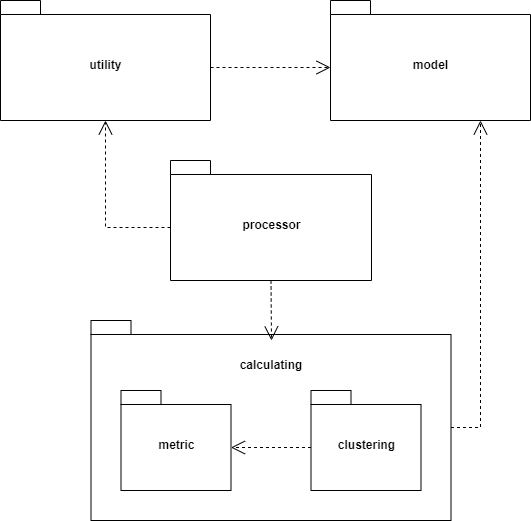
\includegraphics[width=\textwidth]{packages.png}
    \end{center}
    \caption{Paketdiagramm des Tools.}
    \label{fig:Packages}
\end{figure}

\clearpage
\section{Programmablauf}
\label{4-Programmablauf}
Im Folgenden wird der Programmablauf beschrieben.
\begin{enumerate}
    \item Der Nutzer startet den \emph{Processor}
    und gibt als Startparameter den Pfad der \emph{config-Datei} an.
    \item Der \emph{Processor} nutzt den \emph{Config-Reader}, um die Werte der \emph{Konfigurationdatei} auszulesen
    und speichert diese ab.
    \item Der \emph{Processor} nutzt den \emph{DataReader}, um den Datensatz einzulesen
    und legt die Informationen in geeigneten Objekten ab.
    Für den Kinect-Datensatz sind die Implementierungen \emph{RecordImpl} und \emph{FrameImpl}
    bereitgestellt.
    \item Der \emph{Processor} startet das Clustering durch den Aufruf der \emph{cluster-Methode}
    eines \emph{HierarchicalClustering-Objekts}.
    Zu beginn entspricht jeder Record einem eigenen Cluster.
    Die \emph{recordToCluster-Methode} ermöglicht eine Transformation von Records zu Clustern.
    \item Das Clustering nutzt ein \emph{\ac{DTW}-Objekt},
    um paarweise die geringsten Kombinationskosten zweier Cluster zu berechnen.
    \item Die beiden Cluster mit den geringsten Kombinationskosten werden zusammengeführt.
    Konkret wird eines der Cluster in das andere integriert.
    Durch diese Kombination entsteht ein neues Cluster.
    Für alle Attribute werden die Wertereihen für das neue Cluster aus denen der alten Cluster berechnet und abgespeichert.
    Zudem werden alle Bestandteile des neuen Clusters abgespeichert.
    Bei allen Komponenten wird zudem ein boolescher Wert auf \emph{false} gesetzt,
    damit sie bei zukünftigen Vergleichen nicht mehr berücksichtigt werden.
    \item Schritte 5 und 6 werden so lange wiederholt, bis die geringsten Kosten den vom Nutzer definierten Threshold übersteigen.
    \item Der \emph{Processor} nutzt den \emph{Cluster-Writer}, um alle Cluster der \emph{clusters-Liste}
    in eine Ausgabedatei zu schreiben.
    \item Der \emph{Processor} nutzt die \emph{VisualizerImpl}, um alle Records der gefundenen Cluster zu visualisieren.
    \item Die Anwendung terminiert. 
\end{enumerate}
